%%%%%%%%%%%%%%%%%%%%%%%%%%%%%%%%%%%%%%%%%%%%%%%%%%%%%%%%%%%%%%%%%%%%%%%%%%%
% Assignment 3.2: Testing for homogeneity of variance by hand
%%%%%%%%%%%%%%%%%%%%%%%%%%%%%%%%%%%%%%%%%%%%%%%%%%%%%%%%%%%%%%%%%%%%%%%%%%%

\handassignment{Assignment 3.2: Testing for homogeneity of variance by hand}

A manufacturer of machines for food processing has created a machine that fills bags with sugar. A machine like this is never perfect and when a 1-kilo bag of sugar is filled there are always small deviations. the actual content of a bag is often a few grams more or less than a kilo. The manufacturer knows these deviations are bigger for new machines but become smaller as the machine is longer used due to better calibration and the smoothing out of the moving parts. To be able to show this to his clients they take a random sample of eight bags of sugar on the first day of the three months the machine is in use and plots the (absolute) weight deviations. \\

The manufacturer wants to use the chart below for a model that shows how much the machine improves over time, but this requires \concept{homogeneity of variances}. The \concept{variance} in month 1 is 0.801 gr, the \concept{variance} in month 2 is 1.113 gr. The \concept{variance} for month 3 has not been calculated yet. \\

\begin{minipage}[t]{0.5\textwidth}
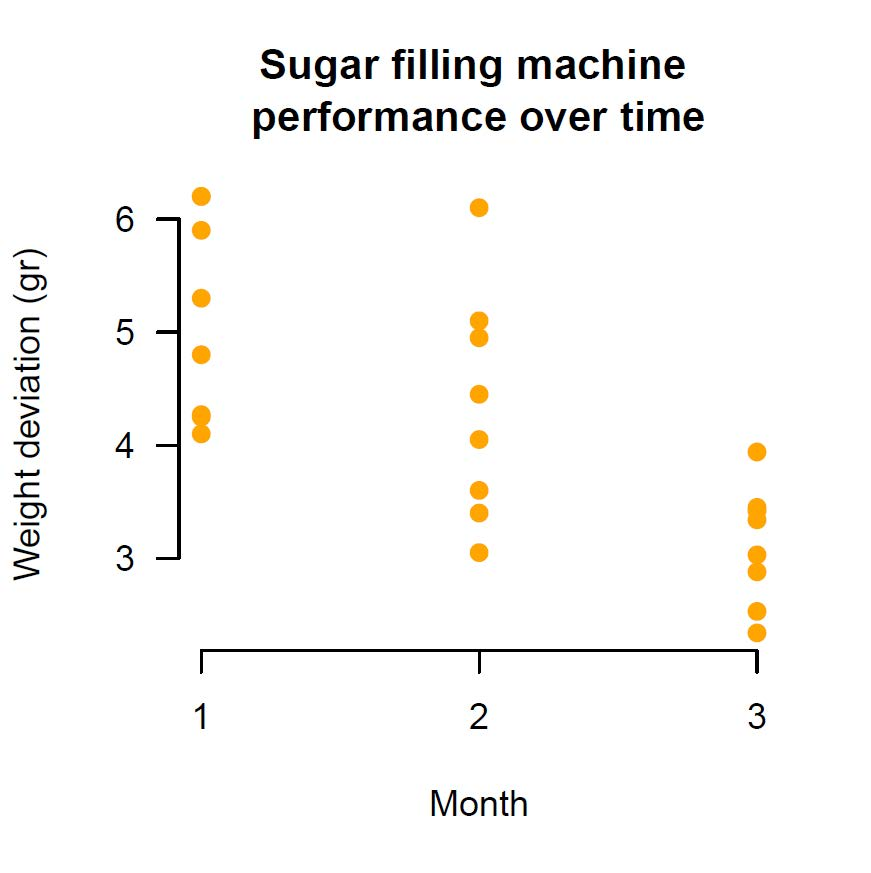
\includegraphics[width=\textwidth]{Files/Images/homogeneityOfVariances.jpg}
\end{minipage}%
\begin{minipage}[t]{0.5\textwidth}
\vspace*{-7cm}
\begin{center}
    \begin{tabular}{|c|c|c|c|}
    \hline 
    $i$ & $x_i$ & $(x_i - \bar{x})$ & $(x_i - \bar{x})^2$ \tstrut\bstrut\\
    \hline
    1 & 3.03 & & \tstrut\bstrut\\
    \hline
    2 & 3.45 & & \tstrut\bstrut\\
    \hline
    3 & 3.94 & & \tstrut\bstrut\\
    \hline
    4 & 2.34 & & \tstrut\bstrut\\
    \hline
    5 & 3.34 & & \tstrut\bstrut\\
    \hline
    6 & 2.53 & & \tstrut\bstrut\\
    \hline
    7 & 2.88 & & \tstrut\bstrut\\
    \hline
    8 & 3.42 & & \tstrut\bstrut\\
    \hline
    \end{tabular}
    \end{center}
    
    $\sum x_i = $  ............. \hspace*{.4cm} $\sum (x_i - \bar{x})^2 = $  ............. \\
    \\
    \hspace*{10pt} $\bar{x} = $ ............. \hspace*{2cm} $s^2 = $  ............. \\
\end{minipage}%

\question{
    3.2 a
}{
    Use the table to the right of the figure to calculate the \concept{variance} $s^2$ for month 3 by filling in the calculations beneath the table.
}

\hint{Hint 3.5: you can find the formula for the \concept{variance} in the formula sheet.}

\emptyanswerbox{
    3.2a
}{
    Variance: \shortanswerline
}   

\question{
    3.2 b
}{
    Calculate \concept{Hartley’s F} (the variance ratio) for the sugar machine data set.
}

\hint{Hint 3.6: you can find the formula for \concept{Hartley’s F} in the formula sheet.}

\clearpage % Page break

\emptyanswerbox{
    3.2b
}{
    Hartley's F: \shortanswerline
}   

\question{
    3.2 c
}{
    Formulate the \concept{null hypothesis} $H_0$ and \concept{alternative hypothesis} $H_1$ to test homogeneity of variance for this case.
}

\hypothesesbox{3.2c}

\question{
    3.2 d
}{
    Determine the \concept{critical value} for Hartley’s F ($F_{\max}$) for the sugar machine data set.
}

\hint{Hint 3.7: Check Table 1 in the formula sheet for the critical values of \concept{Hartley’s F}.}

\emptyanswerbox{
    3.2d
}{
    Hartley's $F_{\max}$: \shortanswerline
}   

\question{
    3.2 e
}{
    Draw the conclusion on the homogeneity of variance for the sugar machine data set. Include the following elements:
    \begin{itemize}
        \item[$\square$] Show how the calculated \concept{Hartley's F} relates to the critical value $F_{max}$.
        \item[$\square$] Discuss whether $H_0$ is rejected or not.
        \item[$\square$] Describe what this tells us about the homogeneity of the three variances.
        \item[$\square$] Describe what type of error is relevant \textit{(type-I or type-II)}.
    \end{itemize}
}

\sixlineanswerbox{3.2e}

\clearpage % Page break